\capitulo{5}{Aspectos relevantes del desarrollo del proyecto}

A la hora de desarrollar el proyecto, nos encontramos con una serie de decisiones a tomar, retos, y cuestiones que tratamos de solucionar a través de formación y aplicación de mejores prácticas. Esta labor fue relativamente sencilla gracias a la disponibilidad de recursos \emph{online} existente hoy en día, así como la participación activa y entusiasmo de la comunidad detrás de las herramientas empleadas en este proyecto.

En este apartado cubrimos los aspectos más destacados en este respecto.

\section{Metodología de desarrollo \emph{software}: Kanban}

El contexto y características en los que se enmarcaba nuestro proyecto son las siguientes:

\vspace{-0.5cm}
\begin{itemize}
	\item [\textbullet] \textbf{Tiempo limitado}: no cabía posibilidad de alargar los plazos, y existían importantes restricciones de tiempo (disponíamos de aproximadamente tres meses para la compleción del proyecto).
	\item [\textbullet] \textbf{Eficiencia y velocidad}: debido a las restricciones mencionadas en el punto anterior, la implementación del proyecto había de ser rápida y eficiente, asegurando siempre un nivel de calidad óptimo.
	\item [\textbullet] \textbf{Motivación y progreso del proyecto}: requeríamos de una metodología que estimulase de manera natural la inversión de tiempo y esfuerzo en el proyecto.
	\item [\textbullet] \textbf{Satisfacción de los usuarios}: dado que ellos son la razón por la que este proyecto se desarrollaba en primer lugar.
\end{itemize}

Atendiendo a los puntos descritos anteriormente, decidimos adoptar un enfoque ágil para el desarrollo de nuestro proyecto. Dentro de las metodologías ágiles, se han consideraron las siguientes:

\begin{itemize}
	\item [\textbullet] \textbf{Scrum}: desarrollo iterativo e incremental centrado en la idea de \emph{sprints}, es decir, iteraciones con una duración fija prefijada, al final de las cuales se produce una entrega parcial del producto.
	\item [\textbullet] \textbf{Kanban}: esta metodología se centra en mantener un flujo constante de trabajo, maximizando la eficencia del equipo de forma que cada tarea sea completada con la mayor celeridad posible.
	\item [\textbullet] \textbf{Programación Extrema (XP)}: se centra en producir \emph{software} de la mejor calidad posible, siendo una de las metodologías ágiles que más profundiza en los aspectos de buenas prácticas de ingeniería para el desarrollo de software.
\end{itemize}

Tras una valoración de las ventajas y desventajas de cada una de estas metodologías, decidimos adoptar la metodología Kanban, gracias también a su mayor flexibilidad. Esto resultó de gran ayuda, dado que, al comenzar este proyecto desconocíamos el funcionamiento concreto de muchas de las herramientas y técnicas utilizadas, por lo que habría sido muy difícil producir ciclos de desarrollo predefinidos y cerrados, como en el caso de Scrum.

No obstante, sí que tomamos ciertos elementos interesantes de esta otra metodología, Scrum, acercándonos en cierto modo a lo que se conoce como Scrumban, una metodología híbrida entre Scrum y Kanban.

A continuación, se recogen las principales características de nuestro sistema de trabajo:

\vspace{-0.5cm}

\begin{itemize}
	\item [\textbullet] Empleamos un tablero Kanban para organizr las historias de usuario, y hacemos uso de instrumentos como los límites WIP (\emph{Work In Progress}) y de herramientas como los Diagramas de Flujo Acumulado (CFD, por sus siglas en inglés).
	\item [\textbullet] Definimos \emph{epics} para agrupar historias de usuario que conformen una misma \emph{feature}, o funcionalidad a desarrollar.
	\item [\textbullet] Debido a la naturaleza de Kanban, no existen \emph{sprints} como tal: el flujo de trabajo es continuo. Sin embargo, sí que se definen tiempos estimados para completar cada tarea (sin emplear puntos de historia; los tiempos se expresan en número de horas empleadas).
	\item [\textbullet] Cada tarea tiene asociada una complejidad, que va desde 0 (mínima complejidad), hasta 10 (máxima complejidad).
	\item [\textbullet] Cada tarea tiene asociada una prioridad. Los niveles de prioridad van desde 0 hasta 3, siendo esta última la prioridad máxima.
	\item [\textbullet] Además del \emph{product backlog}, en el que se recogen las futuras historias de usuario a desarrollar, contamos con otras cuatro columnas: \emph{preparado}, \emph{trabajo en progreso}, \emph{testing}, y \emph{finalizado}.
	\item [\textbullet] Periódicamente, se llevaron a cabo \emph{revisiones} y \emph{retrospectivas}, en las que participaron los tutores.
\end{itemize}

\vspace{-0.2cm}
\begin{figure}[h]
	\centering
	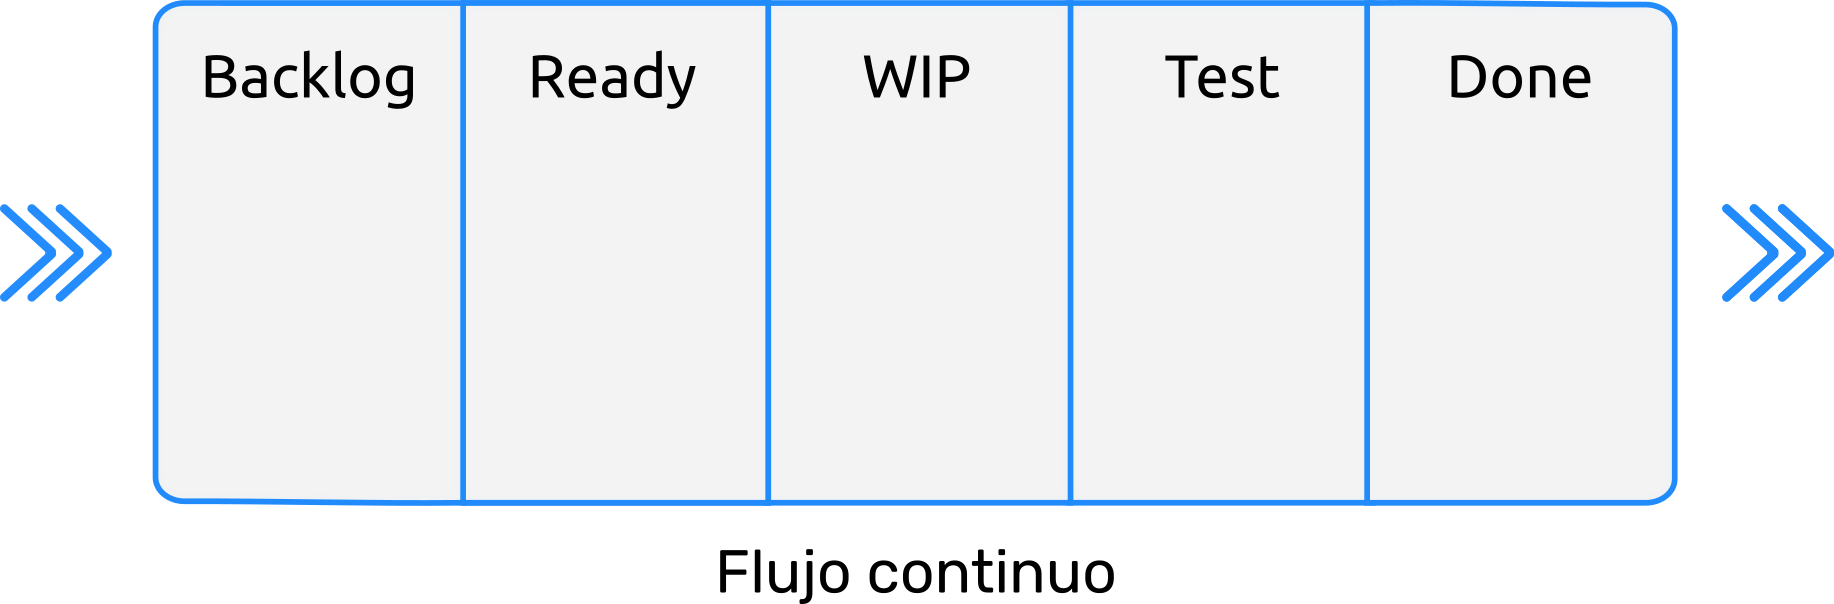
\includegraphics[width=0.8\textwidth]{kanban}
	\caption{Tablero Kanban utilizado.}
\end{figure}

Como herramienta de gestión Kanban, empleamos Kanboard \cite{kanboard}. Se trata de una aplicación \emph{web} \emph{open-source} activamente desarrollada. Contratamos un servidor EC2 con Amazon Web Services (AWS) desde el cual podemos servir la aplicación \emph{web}, la cual a su vez hace uso de una base de datos PostgreSQL en la cual almacena los datos generados. Dicha base de datos está desplegada a través del servicio RDS, también perteneciente a1 AWS.

Se puede acceder al tablero público a través de \href{https://kanban.jizt.it}{\texttt{https://kanban.jizt.it}}.



\section{Motivación tras las arquitecturas desarrolladas}

\subsection{Arquitectura de microservicios}

Desde un primer momento, se concibió la arquitectura con los siguientes objetivos presentes:

\vspace{-0.5cm}
\begin{itemize}
	\item [\textbullet] \textbf{Flexibilidad}: la Inteligencia Artificial y, en concreto, el Procesamiento de Lenguaje Natural, son campos en continuo desarrollo. Cada pocos meses aparecen modelos más potentes que proporcionan mejores resultados. Es por ello que nuestra arquitectura debe proporcionar una estructura lo más desacoplada como sea posible de los modelos concretos de NLP que empleados. De este modo, si aparecieran modelos más avanzados, la transición de unos modelos a otros resultará una labor relativamente sencilla.
	\item [\textbullet] \textbf{Escalabilidad}: los elementos que conforman la arquitectura, deben tener la capacidad de replicarse a fin de responder correctamente a la demanda de usuarios. Adicionalmente, como se ha venido mencionado a lo largo de esta memoria, la implementación de otras tareas de NLP diferentes de la generación de resúmenes es algo que entra dentro de nuestros planes a medio plazo. La arquitectura debe estar estructurada de tal forma que esta expansión se pueda llevar a cabo sin inconvenientes. 
	\item [\textbullet] \textbf{Alta disponibilidad}: relacionada con el punto anterior, se debe poder prestar servicio de forma continua, independientemente de que se produzcan picos en la carga de trabajo, o de que alguno de los componentes falle en un momento dado.
	\item [\textbullet] \textbf{\emph{Cloud native}}: este punto engloba a todos los anteriores; los sistemas \emph{cloud-native} están diseñados para adaptarse a entornos cambiantes, operar a gran escala y poseer resiliencia \cite{cloud20}.
\end{itemize}

Una de las arquitecturas que permiten conseguir los objetivos recogidos anteriormente, es la \textbf{arquitectura de microservicios}. Con este patrón arquitectónico, la aplicación se divide en pequeños servicios, cada uno de los cuales cumple una labor específica, y encapsula todas sus dependencias, a fin de conseguir el máximo grado de independencia posible.

En nuestro caso, además, existen tareas que llevan considerablemente más tiempo que otras, como es el caso de la generación del resumen (que puede durar segundos), frente al pre-procesado del texto (el cual es instantáneo). Una arquitectura como esta nos permite replicar el microservicio encargado de la generación del resumen, para repartir la carga de trabajo entre las diferentes réplicas.

Además, si uno de los microservicios fallara, sería reemplazado inmediatamente por una nueva réplica, gracias a la tecnología de Kubernetes.

\subsection{Arquitectura dirigida por eventos}

Dado que ya ha sido introducida en la \hyperref[subsec:kafka]{sección referente a Kafka}, no entraremos en mucho detalle para evitar repetirnos.

Simplemente recordaremos que este patrón arquitectónico hace posible la comunicación entre los microservicios de forma fiable y rápida. En nuestro caso, un evento sería la finalización del trabajo por parte de uno de los microservicios. Este evento genera una respuesta en otro de los microservicios, el cual lo procesa y comienza su labor específica.

Este patrón nos ofrece también flexibilidad a la hora de introducir nuevos microservicios, ya que, al menos en el caso de Kafka, el \emph{topic} al que un microservicio produce (o consume) eventos podría ser modificado en tiempo de ejecución, sin necesidad de alterar el código fuente del microservicio.

\subsection{API REST Asíncrona}

La generación de resúmenes es un proceso que se puede dilatar varios segundos en el tiempo, dependiendo de factores como la longitud del texto o de los parámetros con los que se genere el resumen. Por lo tanto, realizar peticiones síncronas queda descartado, puesto que una petición HTTP no debe prolongarse durante tanto tiempo.

La forma común de solucionar este problema, logrando asincronismo, pasa por realizar una primera petición dándole a conocer al sistema que queremos generar un resumen. El sistema, entonces, responderá haciéndonos saber que la petición ha sido recibida y se está procesando. A partir de ese momento, consultaremos periódicamente al sistema para conocer el estado del resumen, hasta finalmente obtenerlo, una vez haya sido generado.

Veamos el proceso de manera un poco más detallada.

\subsubsection{1. Petición HTTP POST}

El cliente comienza realizando una petición \texttt{POST} incluyendo en el cuerpo de la misma el texto que quiere resumir. La API le responde con un identificador único del resumen, el \texttt{summary\_id}, así como otros campos de interés:

\begin{figure}[h]
	\centering
	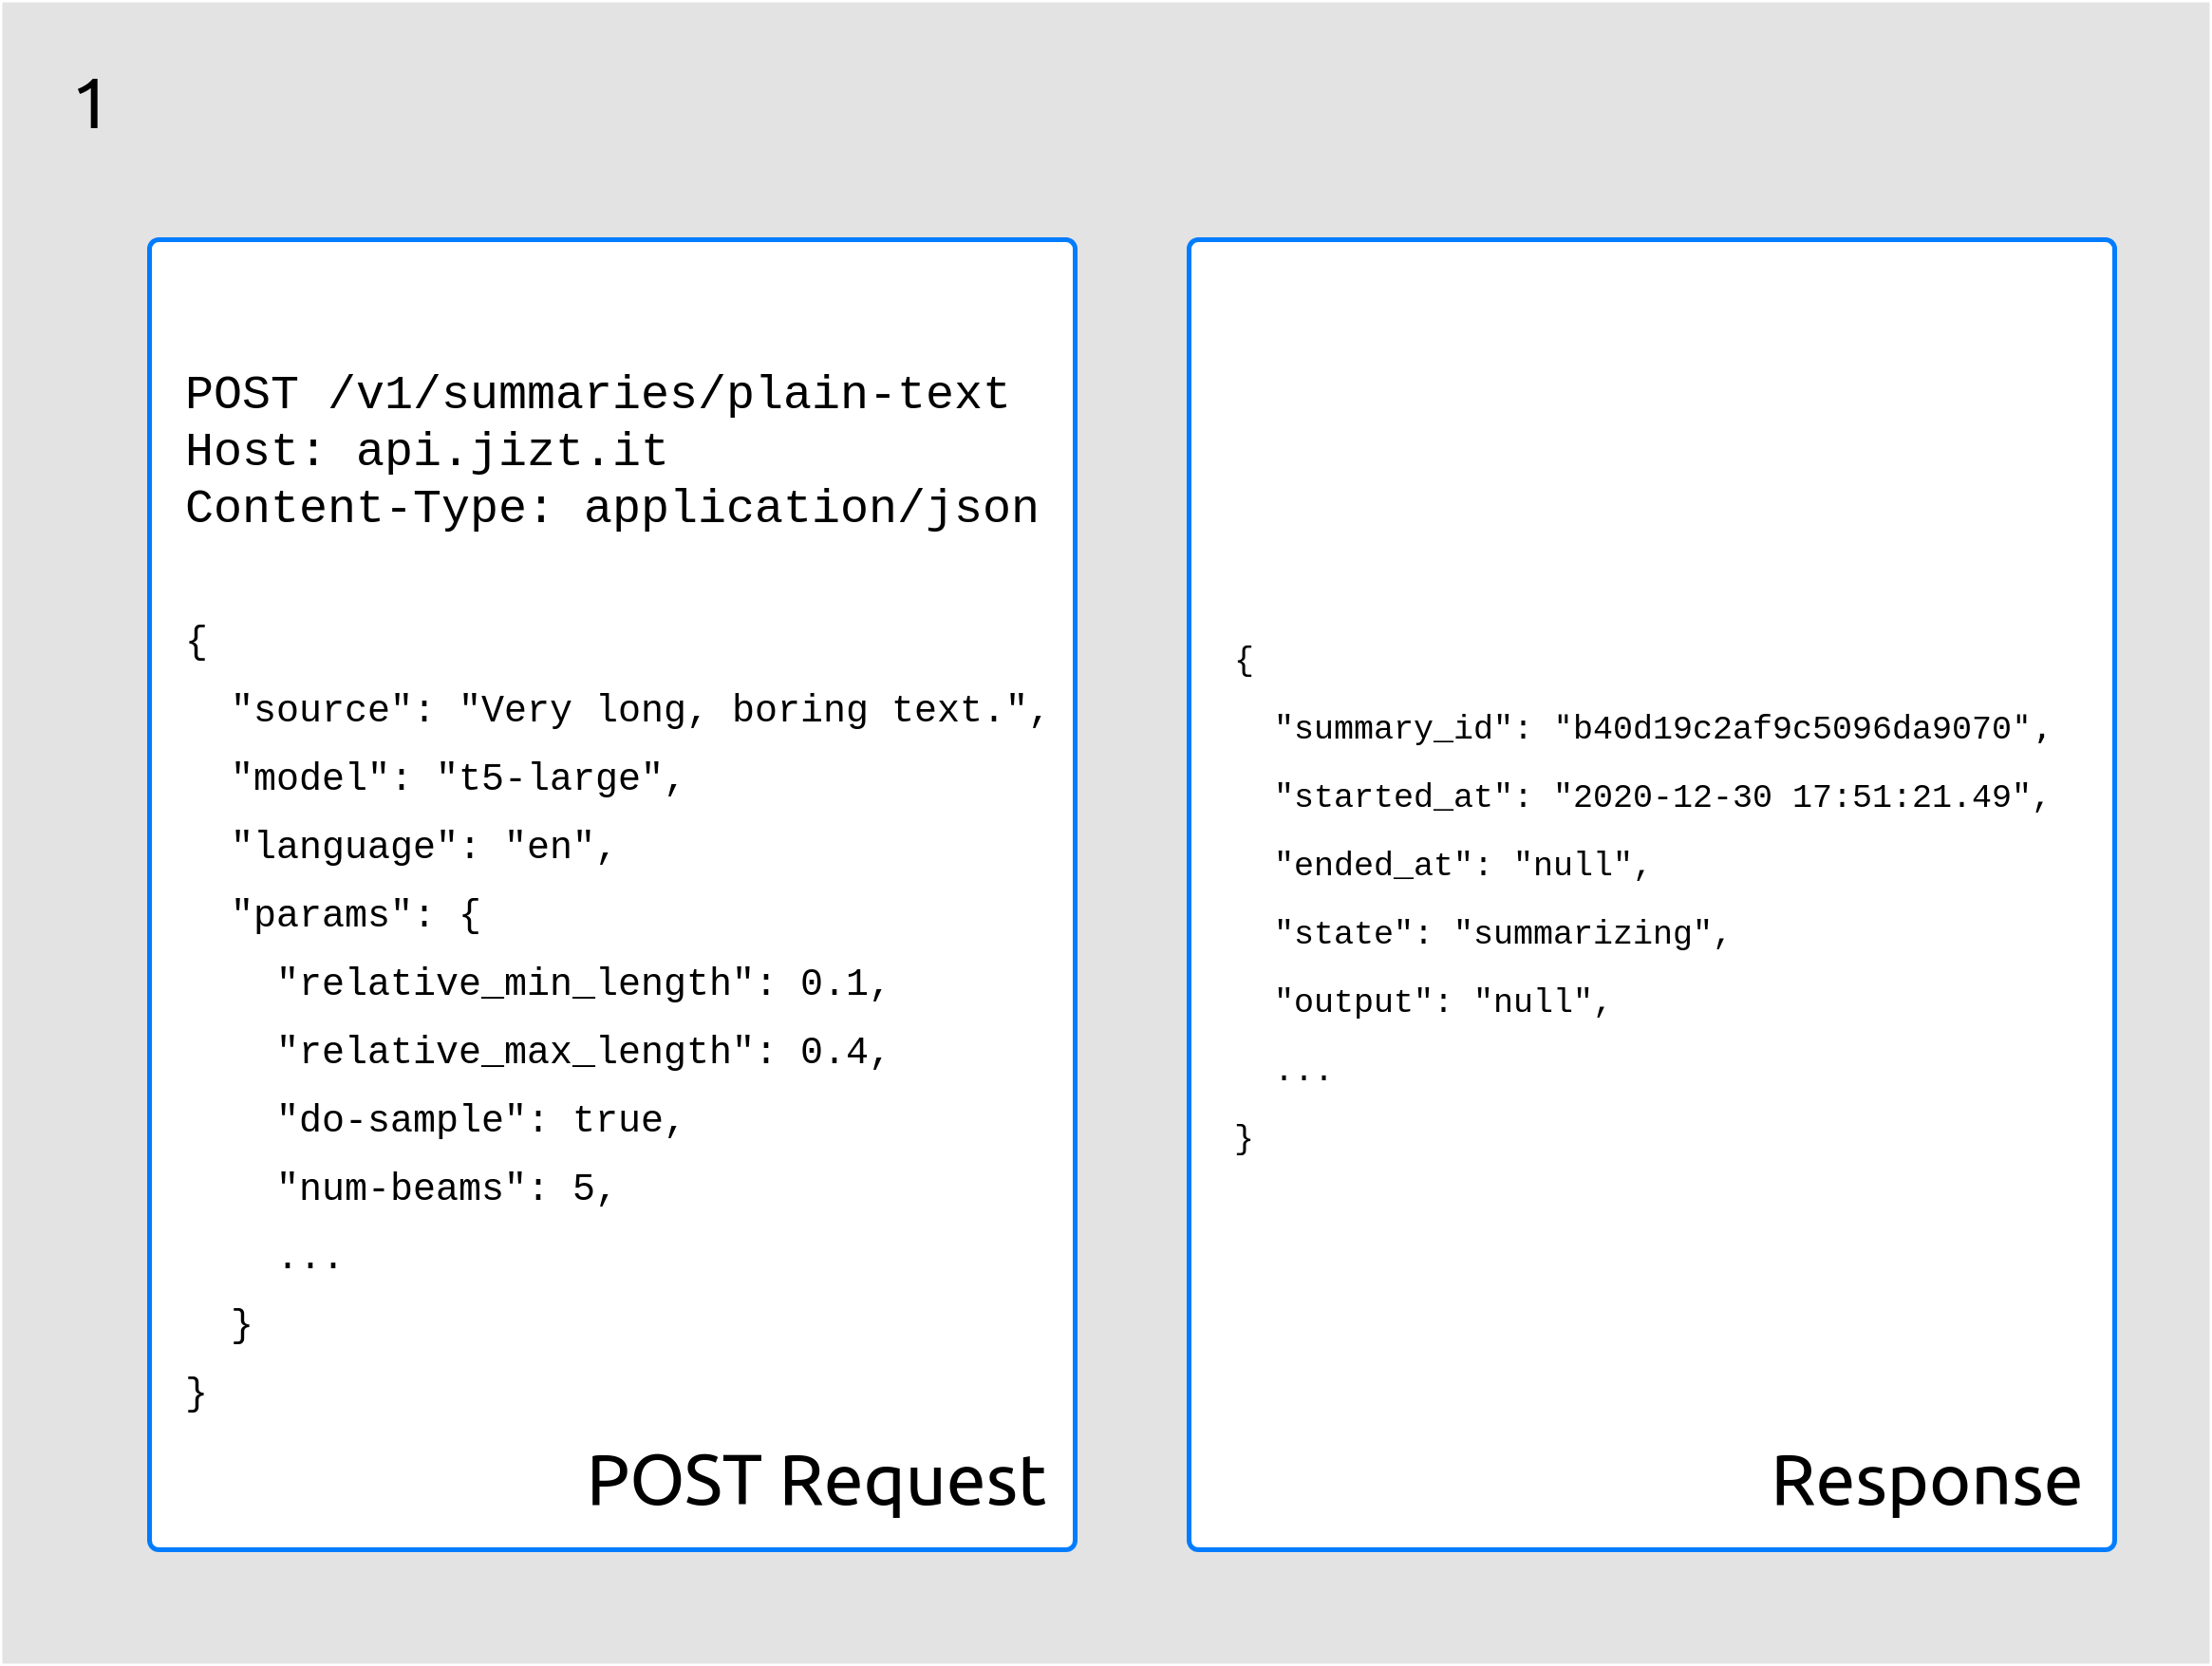
\includegraphics[width=\textwidth]{api-request-1}
	\caption[Primer paso: realizar una petición POST.]{El primer paso es realizar una petición \texttt{POST} con el texto a resumir.}
	\label{fig:api-primer-paso}
\end{figure}

Como vemos en la \hyperref[fig:api-primer-paso]{anterior figura}, el estado del resumen es \texttt{``resumiendo''} (\texttt{``summarizing''}), y aún no tenemos acceso al resumen (\texttt{ouput}), el cual es por el momento \texttt{``null''}.

Una de las principales ventajas de poder consultar el estado del resumen, es poder ofrecer al usuario retroalimentación de los pasos que se están llevando a cabo, mostrándole así que su resumen efectivamente está siendo procesado.

\subsubsection{2. Peticiones HTTP GET sucesivas}

En ese momento, el cliente puede llevar a cabo peticiones HTTP GET con el \emph{id} del resumen de manera periódica a fin de consultar el estado del mismo.

En algún momento, el estado del resumen pasará a ser \texttt{``completado''} (\texttt{``completed''}), y la respuesta a nuestra petición contendrá el resumen generado:

\begin{figure}[h]
	\centering
	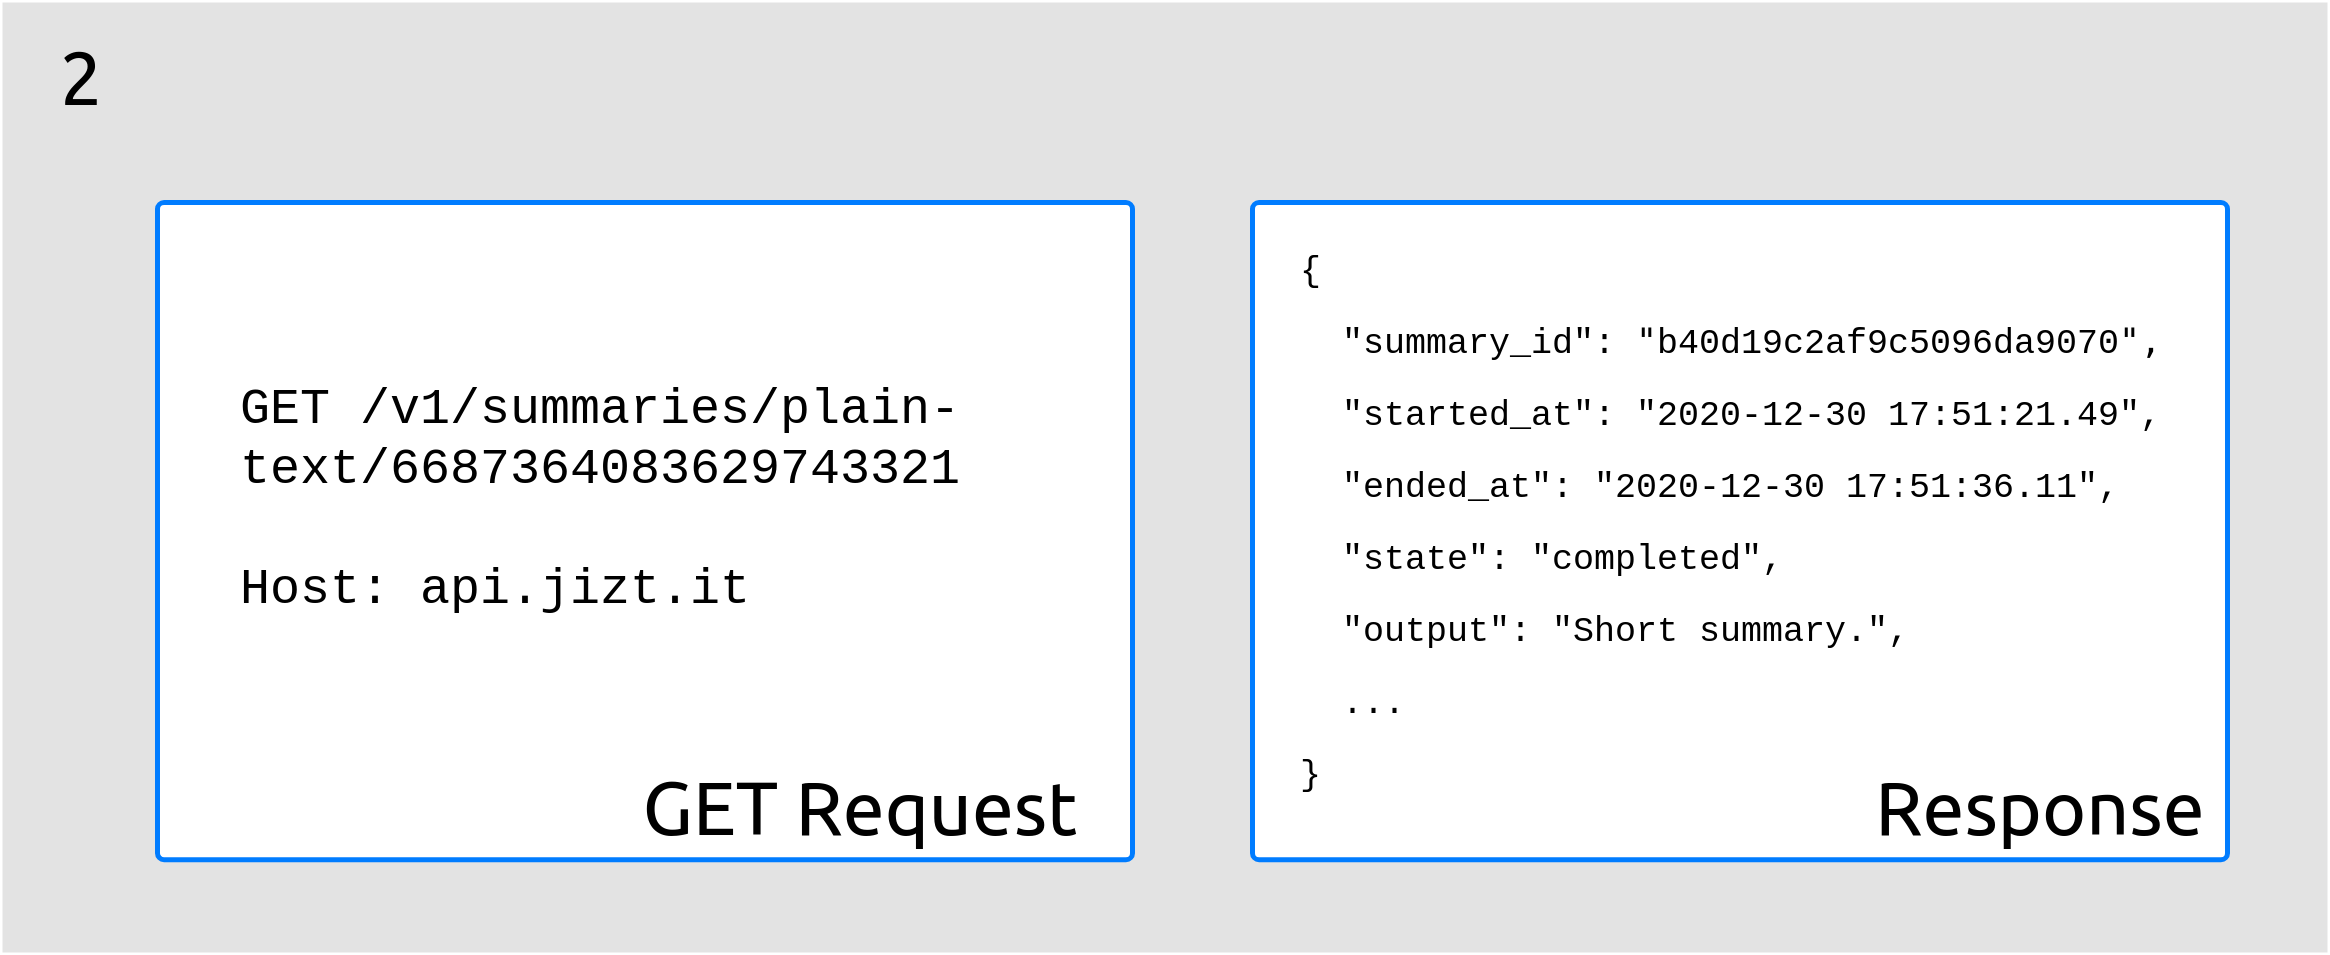
\includegraphics[width=\textwidth]{api-request-2}
	\caption{Finalmente, obtenemos el resumen generado.}
\end{figure}

En el caso de que previamente se hubiera solicitado un resumen del mismo texto, con el mismo modelo y parámetros, el resumen ya estaría almacenado en la base de datos, por lo que la respuesta al primer \texttt{POST} ya contendría dicho resumen.


\subsection{Desarrollo de la aplicación}

A la hora de desarrollar la aplicación, se ha dado gran importancia al diseño de la arquitectura. Con tal fin, nos hemos basado en varios patrones de diseño, dando lugar a una arquitectura que toma elementos de los patrones BLoC \cite{miola20}, \emph{Domain-Driven Design} \cite{vernon13} o \emph{Clean Architecture} \cite{martin15}.

Antes de explicar qué significan estos conceptos, veamos cómo se conforma la arquitectura de la aplicación:

\begin{figure}[!h]
	\centering
	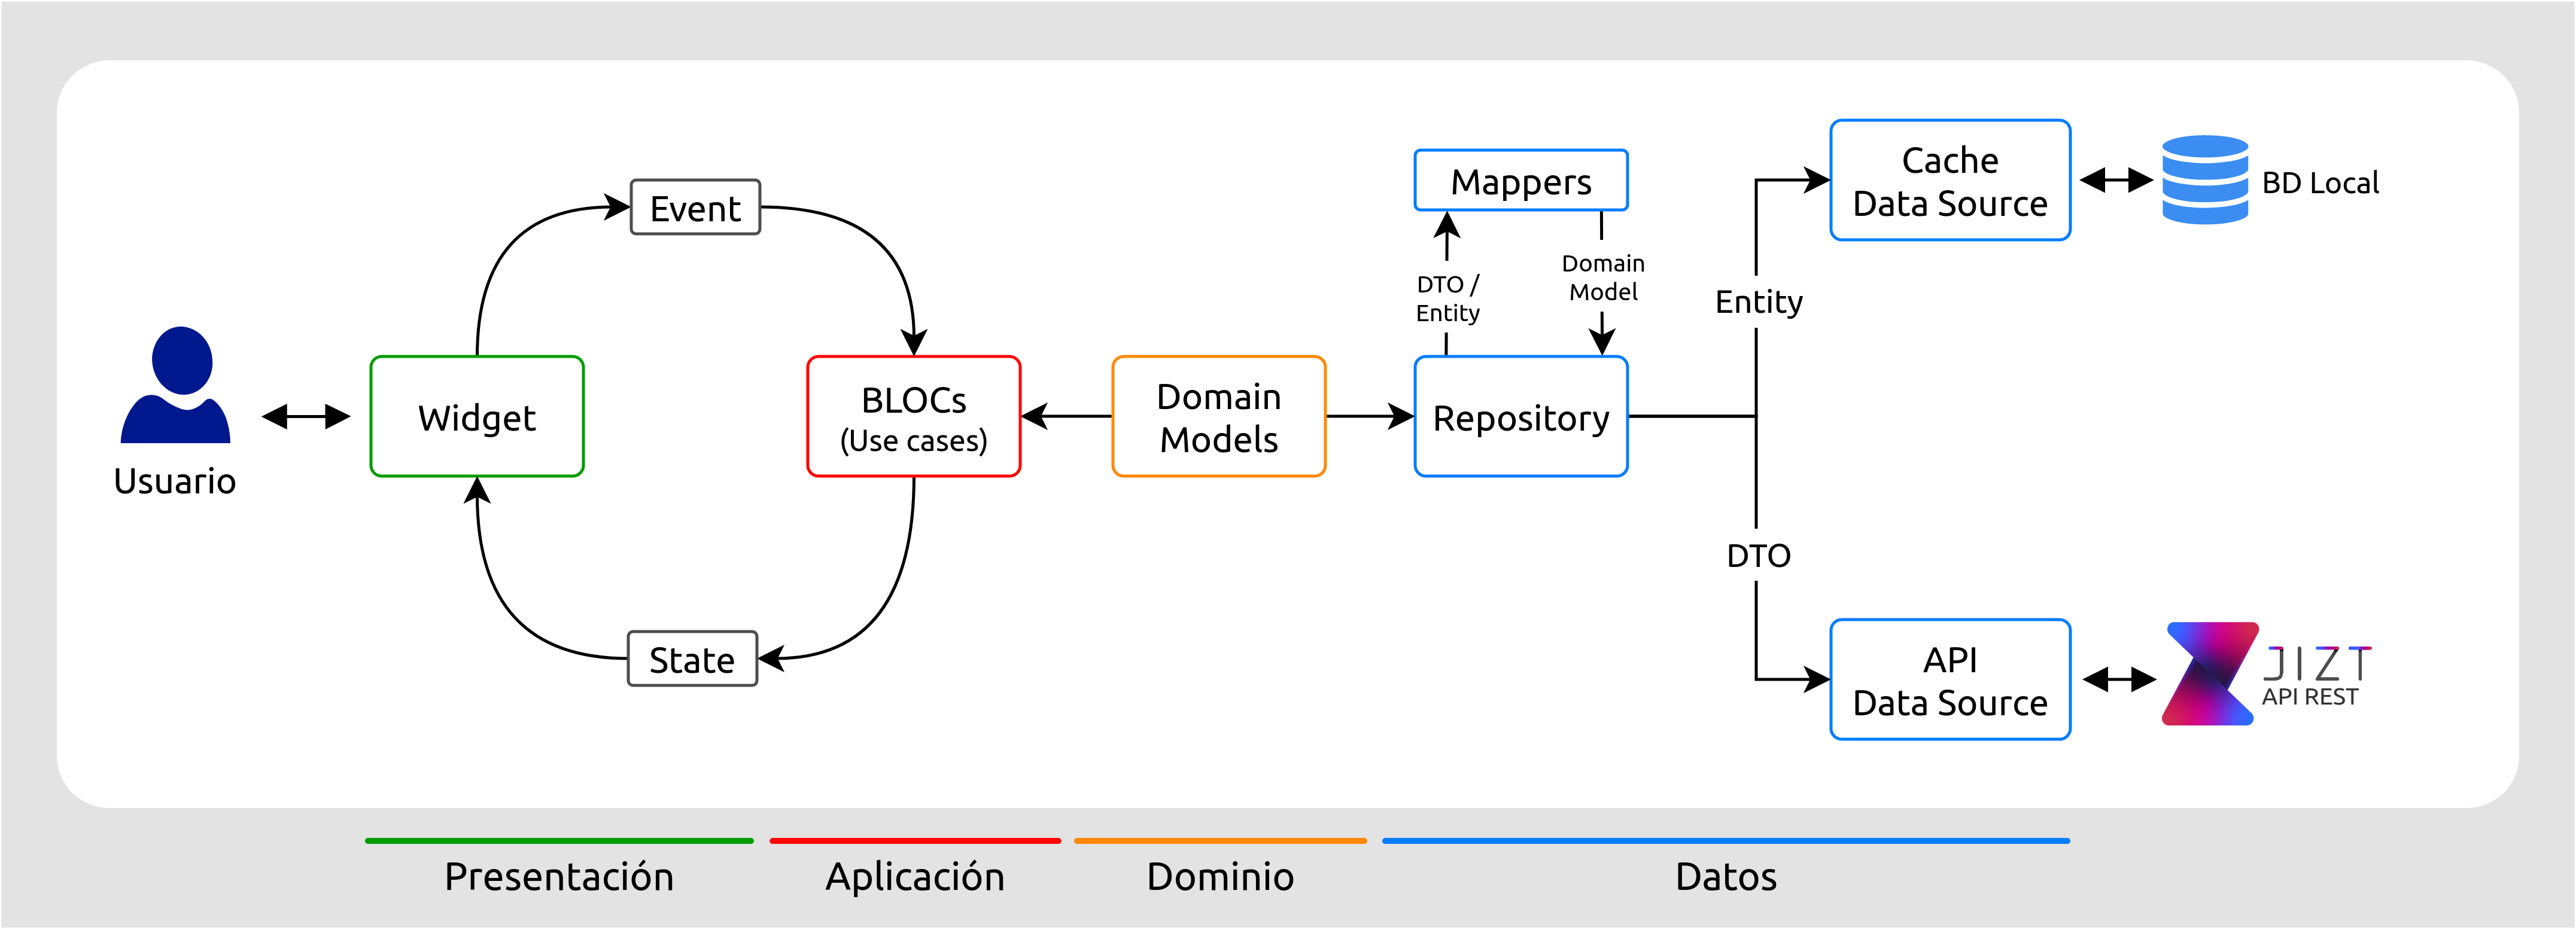
\includegraphics[width=\textwidth]{jizt-app-arch}
	\caption{Arquitectura de la aplicación.}
\end{figure}

Como podemos ver, la arquitectura se divide en cuatro capas: presentación, aplicación, dominio y datos, siendo las primeras las más cercanas al usuario.

Expliquemos de forma más detallada cada una de ellas, comenzando por la capa de \emph{datos}, a la derecha de la imagen.

\subsubsection{Capa de datos}

En esta capa se hace uso del patrón repositorio, el cual sitúa un componente intermedio entre la capa de dominio y el mapeo de los datos a fin de aislar los objetos del dominio de los detalles de implementación concretos a la hora de acceder a la fuente de datos \cite{vernon13}.

Nuestra aplicación implementa un caché local, de forma que, cuando el usuario solicita un resumen, se comprueba primero si dicho resumen ya ha sido generado previamente, acudiendo a la base de datos local, y en caso afirmativo, se recupera directamente el resumen; si no, se aguarda a la respuesta de la API REST.

Esta capa es el punto de conexión entre tres ámbitos  diferentes: la capa de dominio, la cual explicaremos a continuación, la caché local, y la API REST.

La forma en que cada uno de estos ámbitos represente los datos (en nuestro caso, los resúmenes) es independiente del resto. Por ello, vamos a contar con tres representaciones diferentes, cada una correspondiéndose con uno de los ámbitos descritos:

\begin{itemize}[\textbullet]
	\item \emph{Domain Model}: es la representación de los resúmenes propia de la capa de dominio.
	\item DTO (\emph{Data Transfer Object}): se corresponde con la representación del \emph{backend}, esto es, la API REST.
	\item \emph{Entity}: es la representación del caché local.
\end{itemize}

Para que estas tres representaciones diferentes se acoplen correctamente, se hace uso de los \emph{mappers}, los cuales se encargan de transformar la representación de la capa de dominio a DTOs o \emph{Entities}, y viceversa.

\subsubsection{Capa de dominio}

Esta capa define la lógica de negocio de la aplicación, y es independiente de la plataforma de desarrollo, es decir, en nuestro caso estará escrita puramente en Dart, sin contener ningún elemento de Flutter \cite{flutter-clean-arch}. El motivo reside en que el dominio, como decíamos, solo debe ocuparse de la lógica de negocio, y no de los detalles de implementación. Esto también permite una fácil migración entre plataformas, en caso de ser necesario en algún momento.

\subsubsection{Capas de aplicación y presentación}

En estas capas entra en juego el patrón BLoC (\emph{Business Logic Component}). Para entender este patrón, debemos primero explicar los conceptos de \emph{evento} y \emph{estado}.

Dicho de manera sencilla, un estado es aquello que se muestra en la pantalla en un momento específico. Y un evento no es más que una acción detectada por la aplicación, por ejemplo, un \emph{click} del usuario.

Los actores centrales de este patrón son los casos de uso (llamados también BLoCs, como el propio patrón), los cuales contienen las reglas de negocio específicas de la aplicación.

Una vez introducidos los conceptos, podemos identificar cuatro pasos fundamentales:

\vspace{-0.3cm}
\begin{enumerate}
	\item Un componente (\emph{widget}) envía un \emph{evento} al componente BLoC.
	\item El BLoC acepta el evento y lleva a cabo la tarea que tiene asociada, probablemente interaccionando con la capa de dominio.
	\item El BLoC actualiza su \emph{estado}.
	\item Los componentes detectan el cambio de estado y reaccionan de algún modo.
\end{enumerate}

Anteriormente, hemos mencionado el término \emph{widget}. En Flutter, los \emph{widgets} son los elementos que conforman la interfaz de usuario \cite{flutter-widget}, como un botón o un \emph{layout}. Los \emph{widgets} se organizan de forma jerárquica, de modo que toda aplicación tendrá un \emph{widget} raíz, del cual <<colgarán>> el resto de \emph{widgets}, como podemos ver en la \hyperref[flutter-widgets]{siguiente figura}.

\begin{figure}[!h]
	\centering
	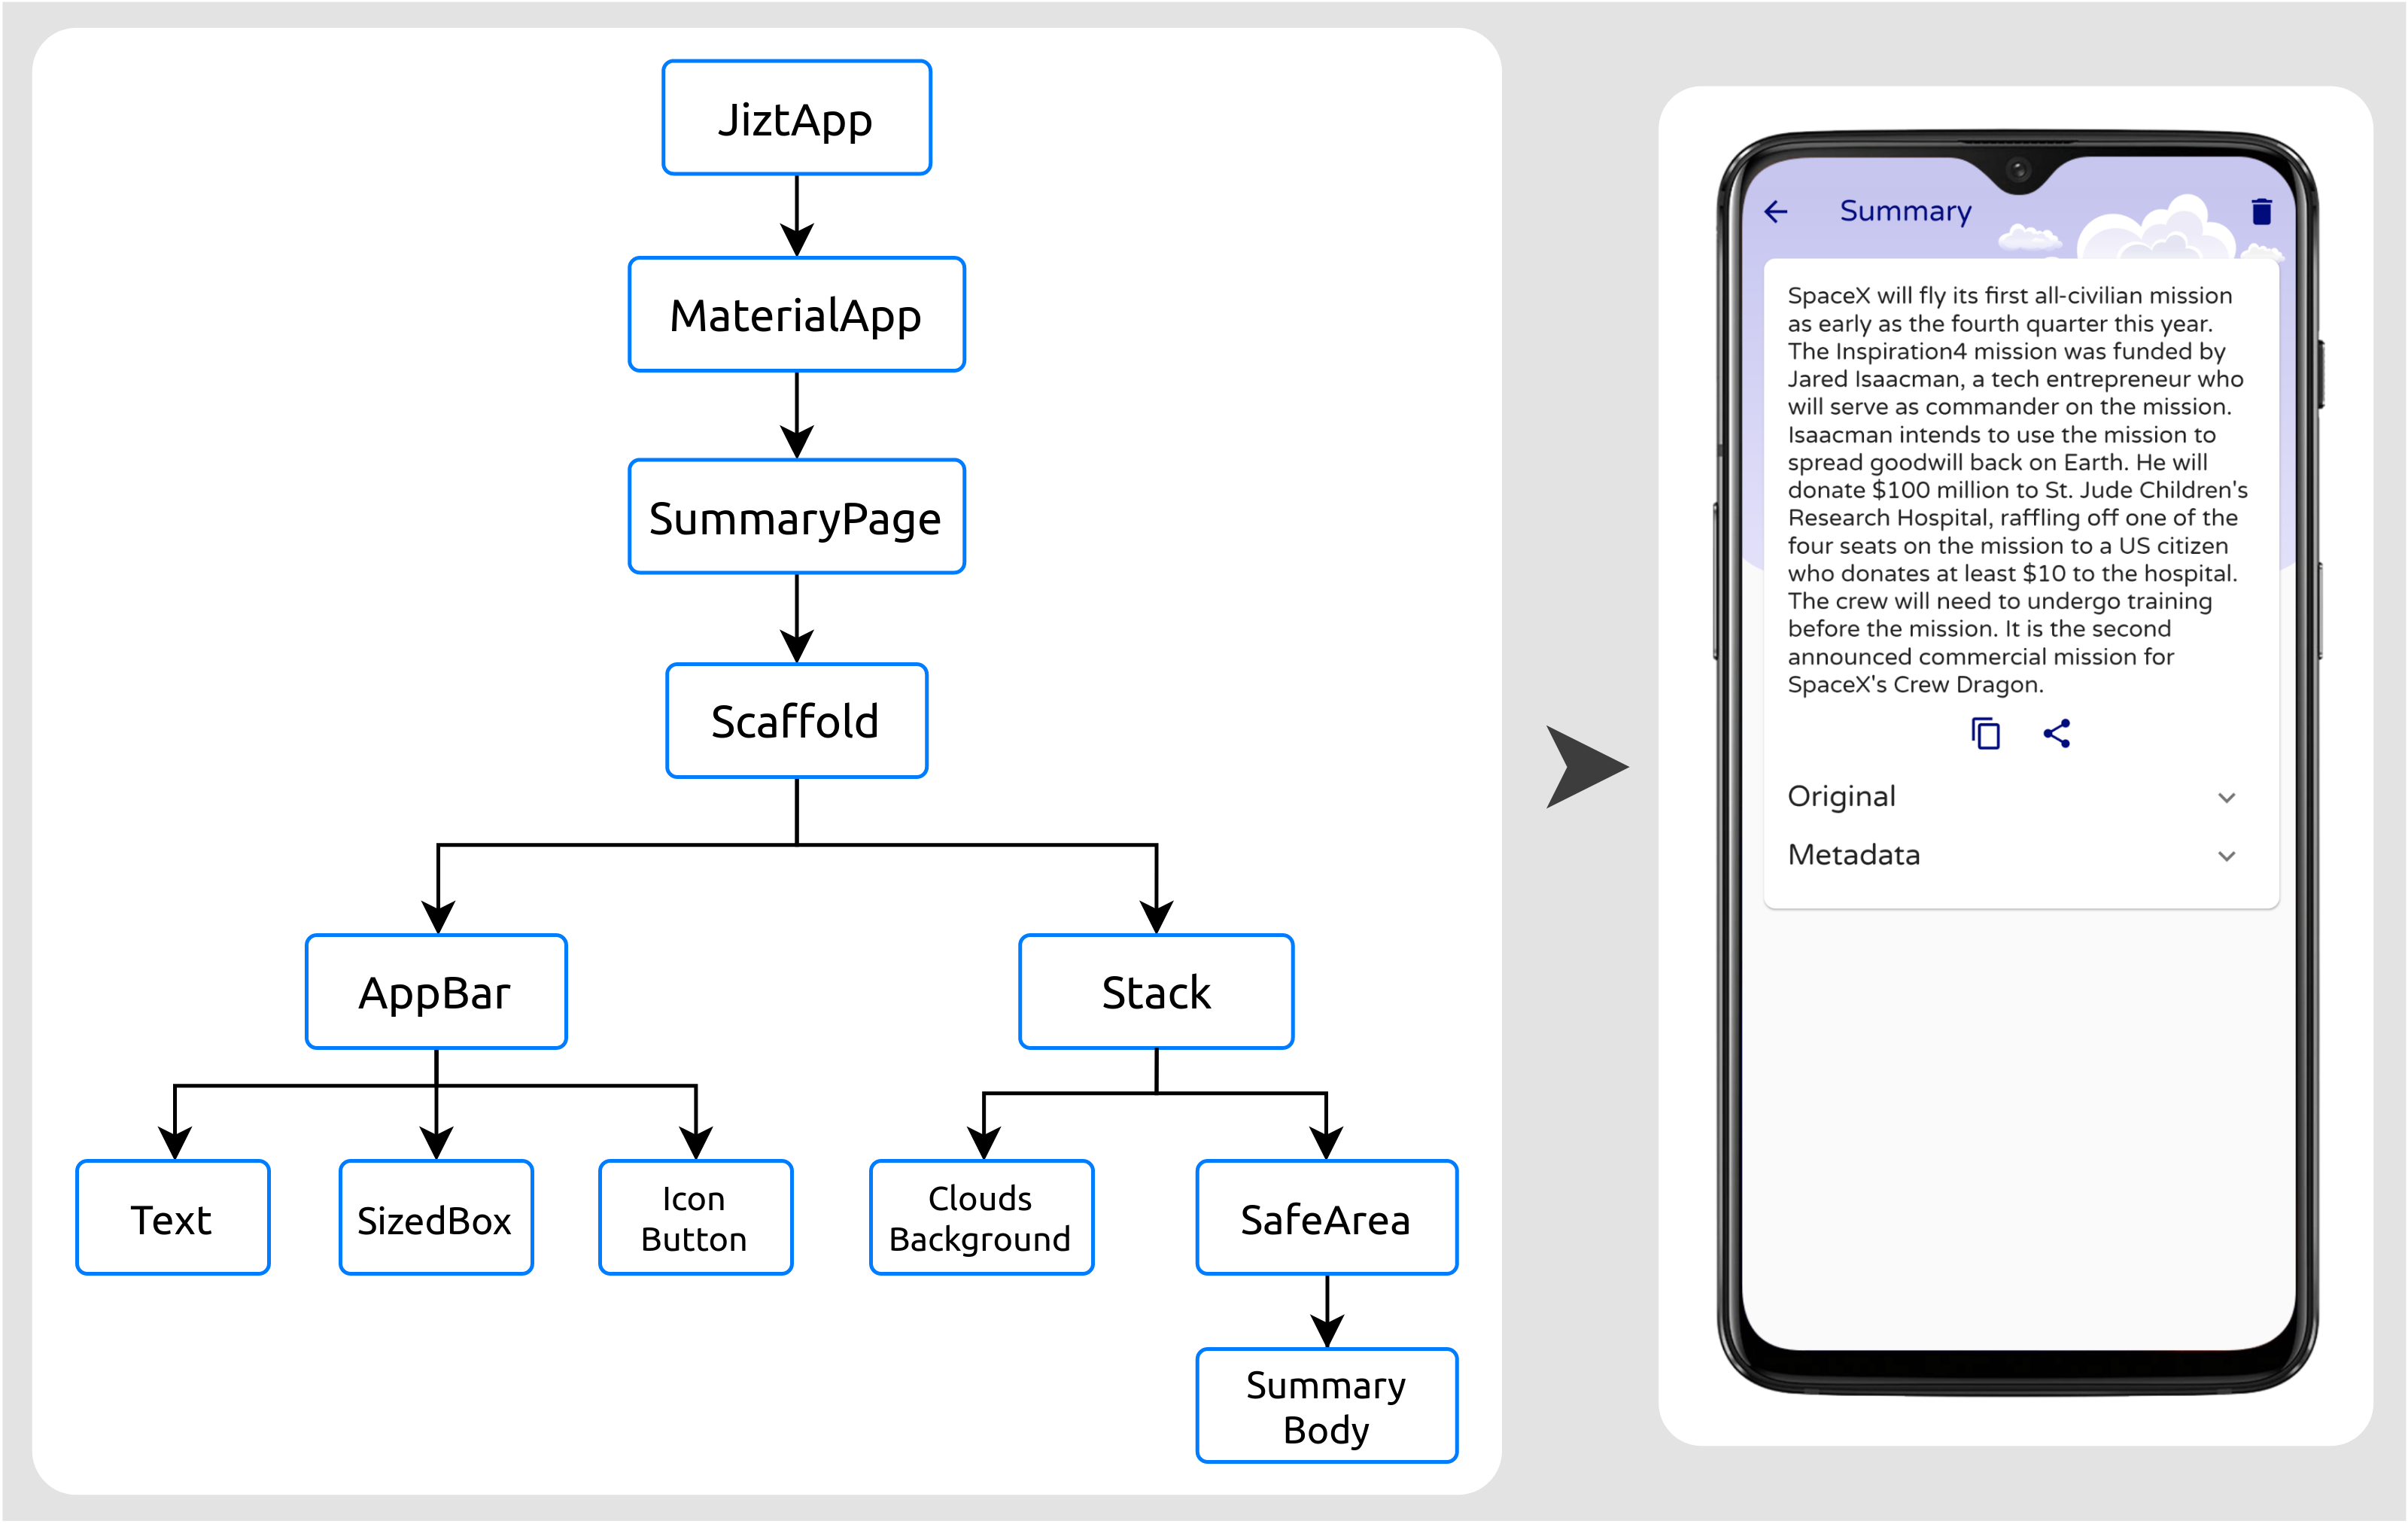
\includegraphics[width=1\textwidth]{widget-hierarchy}
	\caption[Ejemplo de jerarquía de \emph{widgets}.]{Ejemplo de jerarquía de \emph{widgets} de una aplicación sencilla. Imagen del dispositivo móvil extraída de \cite{miola20}.}
	\label{flutter-widgets}
\end{figure}

